\section{Recommendations and Conclusion}
\label{sec:discussion}

When prompted for an overall rating to provide to the system, the users mostly gave the web application 7 or 8 out 10, as Fig \ref{fig:overall} shows. However, a few suggestions came up from the survey, including introducing a passport home delivery system. Some of the users mentioned that the premium service fees were quite high.

\begin{figure}[ht]
\centering
\centerline{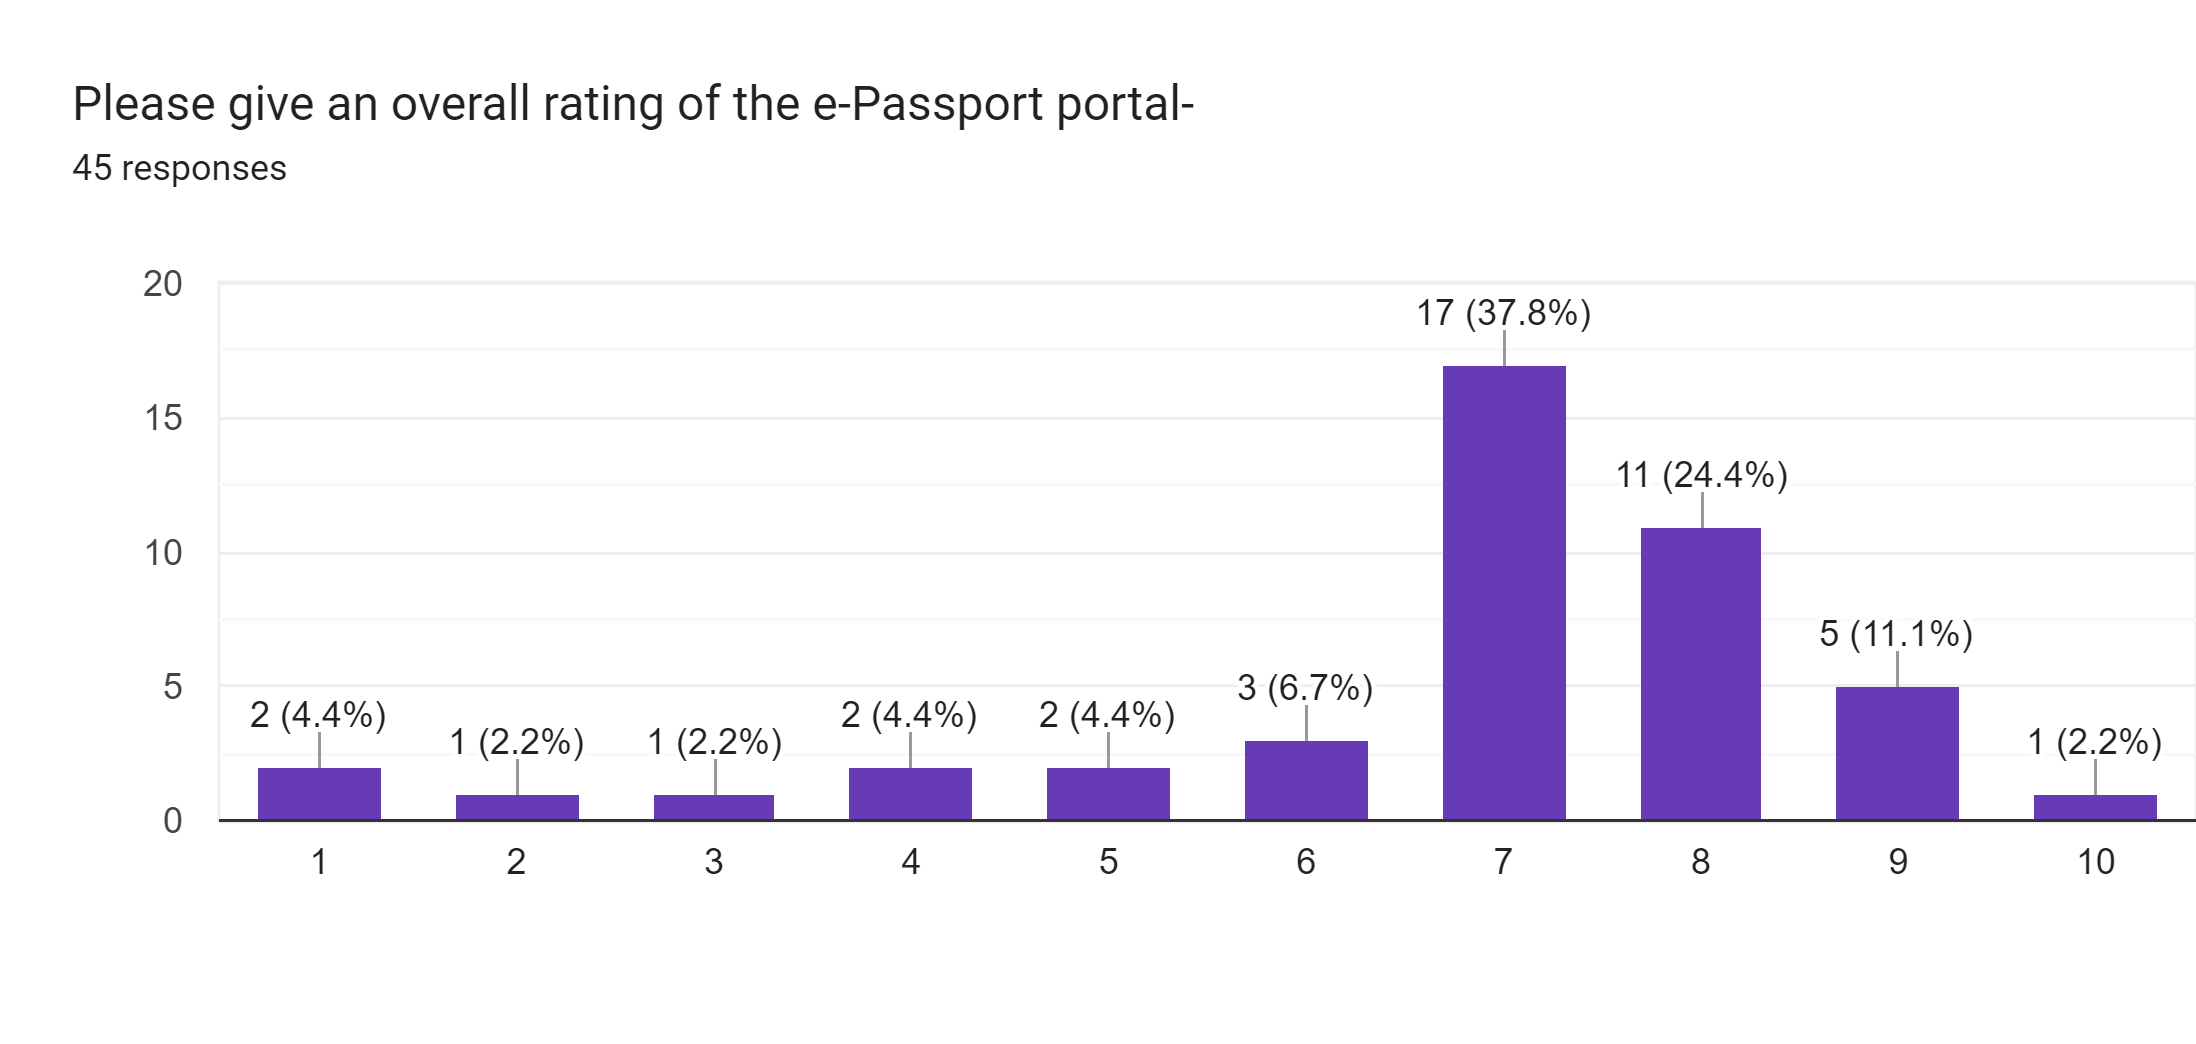
\includegraphics[width=\linewidth]{Figures/overall.png}}
\vspace{-10pt}\caption{Overall rating of the e-Passport portal}
\label{fig:overall}
\end{figure}

We present some suggestions based on the user feedback and 8 golden rules of interface design given by Shneiderman \cite{sp10}:

\begin{itemize}
    \item There should be enough flexibility regarding editing the application and even canceling it even after scheduling in case of emergencies. Easy reversal of actions should be permitted. 
    \item Focus must be increased on effective load balancing. Authorities might give thought to increasing the budget for skilled developers.
    \item The website should be updated on a regular basis to keep the information and instructions up-to-date and complete. 
    \item The payment module can be redesigned as the current one has been performing poorly for quite a period of time. 
    \item Video demonstrations of the application steps can be added to the homepage.
    \item Already existing database entries should be migrated carefully within the scope of the website so that renewal cases do not require filling up the same information again.
    \item Application progress summary can be shown in a sidebar as one proceeds through different sections of the form, effectively reducing the short-term of the user.
    \item The contact and feedback sections need to be improved. A dedicated help desk should be formed and monitored to be active. Feedback initiatives are recommended to be more frequent and to the point.
\end{itemize} 

Addressing the issues presented in this article will hopefully make the e-passport portal more user-friendly and effective enough to serve a large scale of people over the upcoming years.